
\chapter{Willingness to Pay Modeling (WTP): }
\section{The Price-Response Function}
Each price-response function specifies the demand that the lender would experience at each price, which will depend on:
\begin{itemize}
    \item $D$ Number of interested applicants, accepted by the bank's creditworthyness criteria, who would achieve a positive surplus from taking the loan from the lender at the offered price.
    \item $F(p)$ Number of accepted applicants who \textbf{take-up} the offered loan at a given price $p$.
\end{itemize}
In most lending markets, the final price is not known to the client at the time she applies for the loan so we assume that the number of clients who apply for a loan is not influenced by the price.
\begin{align}
d(p)=D\bar{F}(p) \label{eq:demand}
\end{align}
$d(p)$ is the number of the loans offered by a lender that would be taken up at the price p. $D$ is the number of successful applicants for the loan, and $\overline{F}(p)$ is the take-up rate, which is defined as the fraction of successful applicants who will take up the loan at price $p$

\begin{align}
\bar{F}(p)=\int^\infty_p f(w)dw
\end{align}
\section{Segmented vs Join Estimation \label{sec:takeuprate}}
One of the most popular techniques to estimate a WTP model is the logistic regression approach. 
For $n$ segments, the segmented estimation assumes each segments has its own demand function so we need to estimate $2n$ parameters.
\begin{align}
\bar{F_i}(p_i)=\frac{e^{a_i+b_i p_i}}{1+e^{a_i+b_i p_i}} =\frac{1}{1+e^{-a_i-b_i p_i}} = \sigma(a_i+b_ip_i) \label{eq_segmented}
\end{align}
Where $\sigma(x)=\frac{1}{1+e^{-x}}$
For $n$ segments, the join estimation assume we can estimate one single price response function that includes all explanatory variables within it (including price)
\begin{align}
\bar{F}(p_i;x_i)=\frac{1}{1+e^{a+b p_i+\theta^T x_i}} \label{eq_join}
\end{align}
Notice that in the two previous equations there is a subtle difference: In the segmented model (\ref{eq_segmented}), the price coefficient varies with each segment however in (\ref{eq_join}) the price coefficient is the same for all segments. This difference is not restrictive. To ilustrate that, lets consider we want to segment according to 2 features. The client's income (high or low) and its channel preference (digital or physical). These two features define 4 segments\footnote{ Common methods to find relevant segments include Classification Trees and non supervised clustering methods such as K-Means or DBScan}. The segmentation aproach will perform four diferent logistic regressions, one for each segment as shown in Figure (\ref{fig:segmentation})

\begin{figure}[H]
  \centering
    \begin{multicols}{2}
      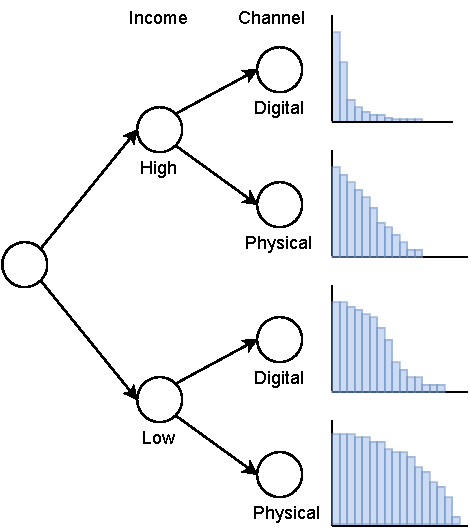
\includegraphics[width=0.43\textwidth]{wtp_segment.pdf} 
    \vfill\null
    \columnbreak
\begin{equation}
    \begin{aligned}
        \bar{F_1}(p) &= \sigma(a_1+b_1p) \\[40pt]
        \bar{F_2}(p) &= \sigma(a_2+b_2p)  \\[40pt]
        \bar{F_3}(p) &= \sigma(a_3+b_3p) \\[40pt]
        \bar{F_4}(p) &= \sigma(a_4+b_4p) 
    \end{aligned} \nonumber
\end{equation}
    \end{multicols}
 \caption{Segmented estimation}
 \label{fig:segmentation}
\end{figure}

A more convenient way to achieve the same models would be to include the segments as another feature in a "bigger" but unique equation. 
\begin{equation}
    \begin{aligned}
    \bar{F}(p) &=& \sigma(a_1I(x_1=\text{H} \wedge x_2=\text{D}) )+b_1 I(x_1=\text{H} \wedge x_2=\text{D}) ) p \\
    & &a_2I(x_1=\text{H} \wedge x_2=\text{P}) )+b_2 I(x_1=\text{H} \wedge x_2=\text{P}) ) p \\
    & &a_3I(x_1=\text{L} \wedge x_2=\text{D}) )+b_3 I(x_1=\text{L} \wedge x_2=\text{D}) ) p \\
    & &a_4I(x_1=\text{L} \wedge x_2=\text{P}) )+b_4 I(x_1=\text{L} \wedge x_2=\text{P}) ) p ) 
    \end{aligned} \label{eq_dummies}
\end{equation}
The decision about wheter to chose one aproach over the other is completely up to the model building team, however if you consider that it is better to work on a systematic framework instead of an ad hoc approach with automation bias you should probably chose the join estimation over the other. Another advantage of the join model is the posibility to learn parameters not only from each individual regression but from the entire data (e.g. lets say we have a digital system which has not much data of volumes -probably because it was only configure to give say \$1000 ticket loans- by generating the joint model we will be able to transfer the learning about the relationship between amount and prices from the other channels and use it to our new channel.
\section{On the flexibility of the logistic function}
To illustrate the shapes the logistic function can take it is useful to express the logistic formula in the form proposed by Richards (1959) \cite{richards-1959} .
\begin{equation}
\bar{F}(x) =\sigma( -b(x-c))  \nonumber
\end{equation}

\begin{figure}[H]
  \centering
    \begin{multicols}{2}
      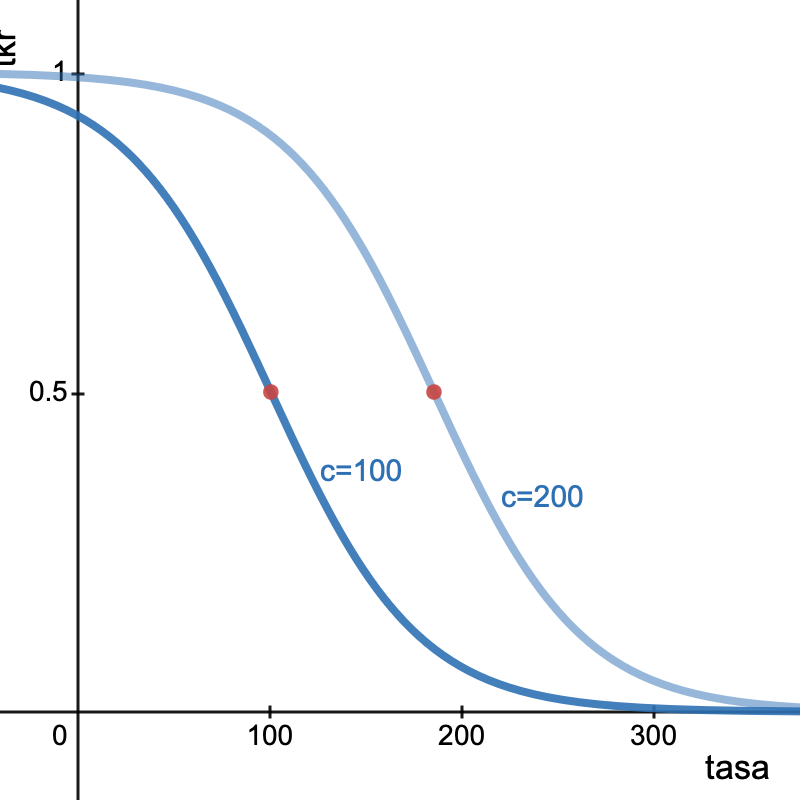
\includegraphics[ width=7cm, height=5cm,
                        ]{desmos-graph1.png} 
    \vfill\null
    \columnbreak
\begin{equation}
    \begin{aligned}
        \bar{F_1}(p) &= \sigma(-b_1(p-100)) \\[40pt]
        \bar{F_2}(p) &= \sigma(-b_2(p-200))  \\[40pt]
    \end{aligned} \nonumber
\end{equation}
    \end{multicols}
 \caption{Center/Bias effect}
 \label{fig:center_shift}
\end{figure}

\begin{figure}[H]
  \centering
    \begin{multicols}{2}
      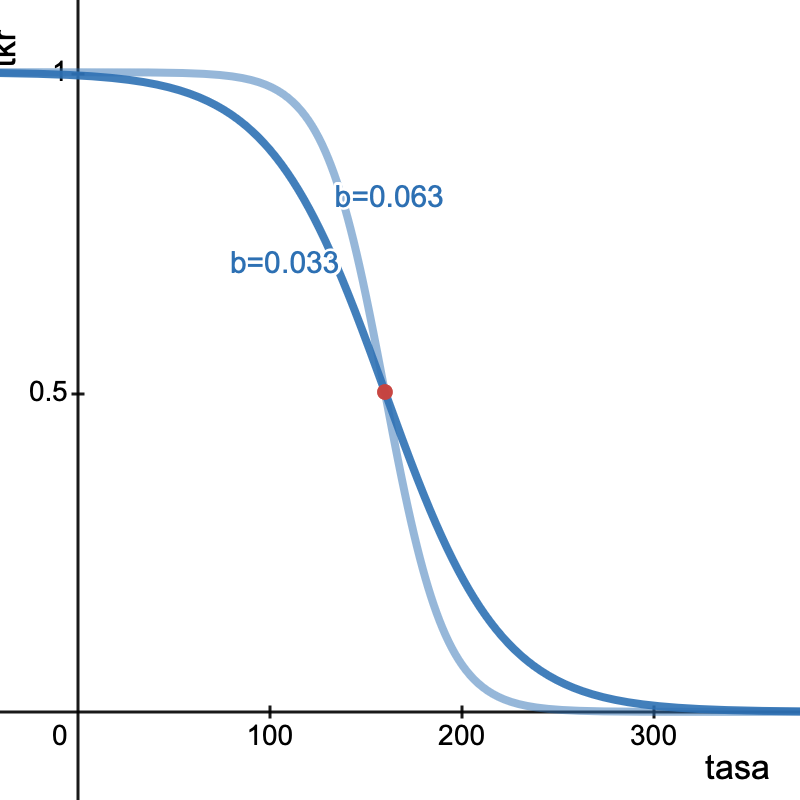
\includegraphics[ width=7cm, height=5cm,
                        ]{desmos-graph2.png} 
    \vfill\null
    \columnbreak
\begin{equation}
    \begin{aligned}
        \bar{F_1}(p) &= \sigma(-0.033(p-150)) \\[40pt]
        \bar{F_2}(p) &= \sigma(-0.063(p-150))  \\[40pt]
    \end{aligned} \nonumber
\end{equation}
    \end{multicols}
 \caption{Pseudo slope effect }
 \label{fig:pslope_shift}
\end{figure}
From the previous analysis we can conclude that if we want to be flexible enough to capture not only differences in the center effect but also the difference in the pseudo slope we should ensure different segments affect not only the intercept coefficient but also the price coefficient. To accomplish that effect a useful specification is the following.
\begin{equation}
     \bar{F}(p) = \sigma(c+x_f^t\beta_f + [p , x_p^t] \beta_p) \label{eqqu}
\end{equation}
Notice that (\ref{eq_dummies}) is a special version of the more general form (\ref{eqqu})
\section{Expected effect of features on client's WTP}

Although the set of variables available for pricing discrimination varies from country to country, we list a set of variables and their expected effects on the WTP for each customer since. \\

Price: The effect of an increase in interest rate is a decrease in the take-up probability. The degree to which this effect takes place is given by the price elasticity. \footnote{Common counter examples include Giffen goods: The scottish economist Robert Giffen, based on his observations of European people in the eighteen century pointed out that when the price of bread rose it drained so much the purchase power of people that they could not afford other goods such as meat and consequently opted out to buy more bread }\\

Amount: Clients expect to receive a better loan offer- a lower rate- when they ask for a bigger ticket. Whenever the bank offers lower rates for bigger ticket there is an incentive for clients to borrow a bigger amount to what is needed and then prepay the excess. This effect can be mitigated for some clients since they will pass first to an underwriting decision process, some clients can qualify for a \$10,000 dollar loan but not for a \$20,000 dollar loan. Another way to mitigate this risk is by capturing the prepayment behavior for these clients into the average prepayment for all portfolio. In this case the rate will be greater for many other clients that will pay for the bad prepayment behavior of a few clients. \\

Channels: A useful framework to assess if clients will have less willingness to pay for a given channel is considering the shopping time available for each client. If the client is known to be operating intensely in digital channels then it is possible that they will have less WTP because they will be more efficient looking at different rates and loan offers, on the other hand, for client who are not so prone to use digital channels they will have less time to spend shopping for rates. \\

Age: The shopping time framework is usefull to shed light about the expected effecto of age, Phillips(2011) \cite{phillips-2021} states that young people and old people tend to have less WTP since they can spend more time shopping for raates whereas middle-aged people have less time to shop so they are more prone to have a higher WTP\\

Income, Geolocation: Any 


\section{Estimation WTP with Black Box Models - Neural Networks}
